% Aberdeen style guide should be followed when using this
% layout. Their template powerpoint slide is used to extract the
% Aberdeen color and logo but is otherwise ignored (it has little or
% no formatting in it anyway).
%
% http://www.abdn.ac.uk/documents/style-guide.pdf

%%%%%%%%%%%%%%%%%%%% Document Class Settings %%%%%%%%%%%%%%%%%%%%%%%%%
% Pick if you want slides, or draft slides (no animations)
%%%%%%%%%%%%%%%%%%%%%%%%%%%%%%%%%%%%%%%%%%%%%%%%%%%%%%%%%%%%%%%%%%%%%%
%Normal document mode
\documentclass[10pt,compress]{beamer}
%Draft or handout mode
%\documentclass[10pt,compress,handout,ignorenonframetext]{beamer}
\newcommand{\frc}{\displaystyle\frac}


%%%%%%%%%%%%%%%%%%%% General Document settings %%%%%%%%%%%%%%%%%%%%%%%
% These settings must be set for each presentation
%%%%%%%%%%%%%%%%%%%%%%%%%%%%%%%%%%%%%%%%%%%%%%%%%%%%%%%%%%%%%%%%%%%%%%
\newcommand{\shortname}{Dr Jeff Gomes}
\newcommand{\fullname}{Dr Jeff Gomes}
\institute{School of Engineering}
\newcommand{\emailaddress}{jefferson.gomes@abdn.ac.uk}
\newcommand{\logoimage}{../FigBanner/UoAHorizBanner}
\title{Module 4: Refrigeration and Liquefaction (EG3539)}
\subtitle{Module 4.2: Gas-Refrigeration Cycles}
\date[18-21/03/2013]{18$^{th}$-21$^{st}$ March 2013}

%%%%%%%%%%%%%%%%%%%% Template settings %%%%%%%%%%%%%%%%%%%%%%%%%%%%%%%
% You shouldn't have to change below this line, unless you want to.
%%%%%%%%%%%%%%%%%%%%%%%%%%%%%%%%%%%%%%%%%%%%%%%%%%%%%%%%%%%%%%%%%%%%%%
\usecolortheme{whale}
\useoutertheme{infolines}

% Use the fading effect for items that are covered on the current
% slide.
\beamertemplatetransparentcovered

% We abuse the author command to place all of the slide information on
% the title page.
\author[\shortname]{%
  \fullname\\\ttfamily{\emailaddress}
}


%At the start of every section, put a slide indicating the contents of the current section.
%\AtBeginSection[] {
%  \begin{frame}
%    \frametitle{Section Outline}
%    \tableofcontents[currentsection]
%  \end{frame}
%}

% Allow the inclusion of movies into the Presentation! At present,
% only the Okular program is capable of playing the movies *IN* the
% presentation.
\usepackage{multimedia}
\usepackage{animate}

%%%%% Color settings
\usepackage{color}
%% The background color for code listings (i.e. example programs)
\definecolor{lbcolor}{rgb}{0.9,0.9,0.9}%
\definecolor{UoARed}{rgb}{0.64706, 0.0, 0.12941}
\definecolor{UoALight}{rgb}{0.85, 0.85, 0.85}
\definecolor{UoALighter}{rgb}{0.92, 0.92, 0.92}
\setbeamercolor{structure}{fg=UoARed} % General background and higlight color
\setbeamercolor{frametitle}{bg=black} % General color
\setbeamercolor{frametitle right}{bg=black} % General color
\setbeamercolor{block body}{bg=UoALighter} % For blocks
\setbeamercolor{structure}{bg=UoALight} % For blocks
% Rounded boxes for blocks
\setbeamertemplate{blocks}[rounded]

%%%%% Font settings
% Aberdeen requires the use of Arial in slides. We can use the
% Helvetica font as its widely available like so
% \usepackage{helvet}
% \renewcommand{\familydefault}{\sfdefault}
% But beamer already uses a sans font, so we will stick with that.

% The size of the font used for the code listings.
\newcommand{\goodsize}{\fontsize{6}{7}\selectfont}

% Extra math packages, symbols and colors. If you're using Latex you
% must be using it for formatting the math!
\usepackage{amscd,amssymb} \usepackage{amsfonts}
\usepackage[mathscr]{eucal} \usepackage{mathrsfs}
\usepackage{latexsym} \usepackage{amsmath} \usepackage{bm}
\usepackage{amsthm} \usepackage{textcomp} \usepackage{eurosym}
% This package provides \cancel{a} and \cancelto{a}{b} to "cancel"
% expressions in math.
\usepackage{cancel}

% Get rid of font warnings as modern LaTaX installations have scalable
% fonts
\usepackage{type1cm} 

%\usepackage{enumitem} % continuous numbering throughout enumerate commands

% For exact placement of images/text on the cover page
\usepackage[absolute]{textpos}
\setlength{\TPHorizModule}{1mm}%sets the textpos unit
\setlength{\TPVertModule}{\TPHorizModule} 

% Source code formatting package
\usepackage{listings}%
\lstset{ backgroundcolor=\color{lbcolor}, tabsize=4,
  numberstyle=\tiny, rulecolor=, language=C++, basicstyle=\goodsize,
  upquote=true, aboveskip={1.5\baselineskip}, columns=fixed,
  showstringspaces=false, extendedchars=true, breaklines=false,
  prebreak = \raisebox{0ex}[0ex][0ex]{\ensuremath{\hookleftarrow}},
  frame=single, showtabs=false, showspaces=false,
  showstringspaces=false, identifierstyle=\ttfamily,
  keywordstyle=\color[rgb]{0,0,1},
  commentstyle=\color[rgb]{0.133,0.545,0.133},
  stringstyle=\color[rgb]{0.627,0.126,0.941}}

% Allows the inclusion of other PDF's into the final PDF. Great for
% attaching tutorial sheets etc.
\usepackage{pdfpages}
\setbeamercolor{background canvas}{bg=}  

% Remove foot note horizontal rules, they occupy too much space on the slide
\renewcommand{\footnoterule}{}

% Force the driver to fix the colors on PDF's which include mixed
% colorspaces and transparency.
\pdfpageattr {/Group << /S /Transparency /I true /CS /DeviceRGB>>}

% Include a graphics, reserve space for it but
% show it on the next frame.
% Parameters:
% #1 Which slide you want it on
% #2 Previous slides
% #3 Options to \includegraphics (optional)
% #4 Name of graphic
\newcommand{\reserveandshow}[4]{%
\phantom{\includegraphics<#2|handout:0>[#3]{#4}}%
\includegraphics<#1>[#3]{#4}%
}

\begin{document}

% Title page layout
\begin{frame}
  \titlepage
  \vfill%
  \begin{center}
    \includegraphics[clip,width=0.8\textwidth]{\logoimage}
  \end{center}
\end{frame}

% Table of contents
%\frame{ \frametitle{Slides Outline}
%  \tableofcontents
%}


%%%%%%%%%%%%%%%%%%%% The Presentation Proper %%%%%%%%%%%%%%%%%%%%%%%%%
% Fill below this line with \begin{frame} commands! It's best to
% always add the fragile option in case you're going to use the
% verbatim environment.
%%%%%%%%%%%%%%%%%%%%%%%%%%%%%%%%%%%%%%%%%%%%%%%%%%%%%%%%%%%%%%%%%%%%%%



%%%
%%%  SECTION
%%%
\section{Gas Refrigeration Cycles}

\subsection{Motivation}
%%%
%%% Slide
%%%
\begin{frame}
 \frametitle{A Few Methods for Refrigeration}
  \begin{enumerate}[(a)]
   \item  Refrigeration by evaporation
   \item \textcolor{blue}{Refrigeration by Expansion of Air}
   \item  Refrigeration by Throttling Process
   \item  Refrigeration using Liquid or Super-critical Gases
   \item  Vapour Refrigeration System
   %\item <6-> 
  \end{enumerate}
\end{frame}


\subsection{Air Standard Gas-Refrigeration Cycles}
%%%
%%% Slide
%%%
\begin{frame}
 \frametitle{Air Standard Cycle}
  \begin{enumerate}[(i)]
   \item <1-> The working fluid in Gas Refrigeration Cycles (GRC) is definitely less complex than in gas power cycles;
   \item <2-> GRC can be either closed or open cycles and obviously it does not involve internal combustion processes, thus;
   \item <3-> Simplified model like the air-standard cycle is lesser necessary. However, many text books adopt simplifications for refrigeration cycles involving gases;
   \item <4-> In particular, all GRCs are assumed to be closed-loop cycles when air-standard cycles analysis is used.
   %\item <6-> 
  \end{enumerate}
\end{frame}

%%%
%%% Slide
%%%
\begin{frame}
 \frametitle{Air Standard Cycle}
   \begin{itemize}
   \item <1-> The following assumptions are usually applied to \textcolor{blue}{gas-refrigeration air-standard cycles} analysis:
  \begin{enumerate}[(a)]
   \item <2-> The working fluid is a fixed mass of air that behaves as an ideal gas;
   \item <3-> All inlet and exhaust processes in open-loop systems are replaced by heat transfer processes to or from the environment;
   \item <4-> All processes within the cycle are reversible;
   \item <5-> The air has constant specific heat capacities.
   %\item <5-> 
   %\item <6-> 
  \end{enumerate}
 \end{itemize}
\end{frame}


\subsection{Reversed Brayton Cycle}
%%%
%%% Slide
%%%
\begin{frame}
 \frametitle{Bell-Coleman Cycle (or Reversed Brayton Cycle)}
    \begin{figure}%
     \begin{center}
      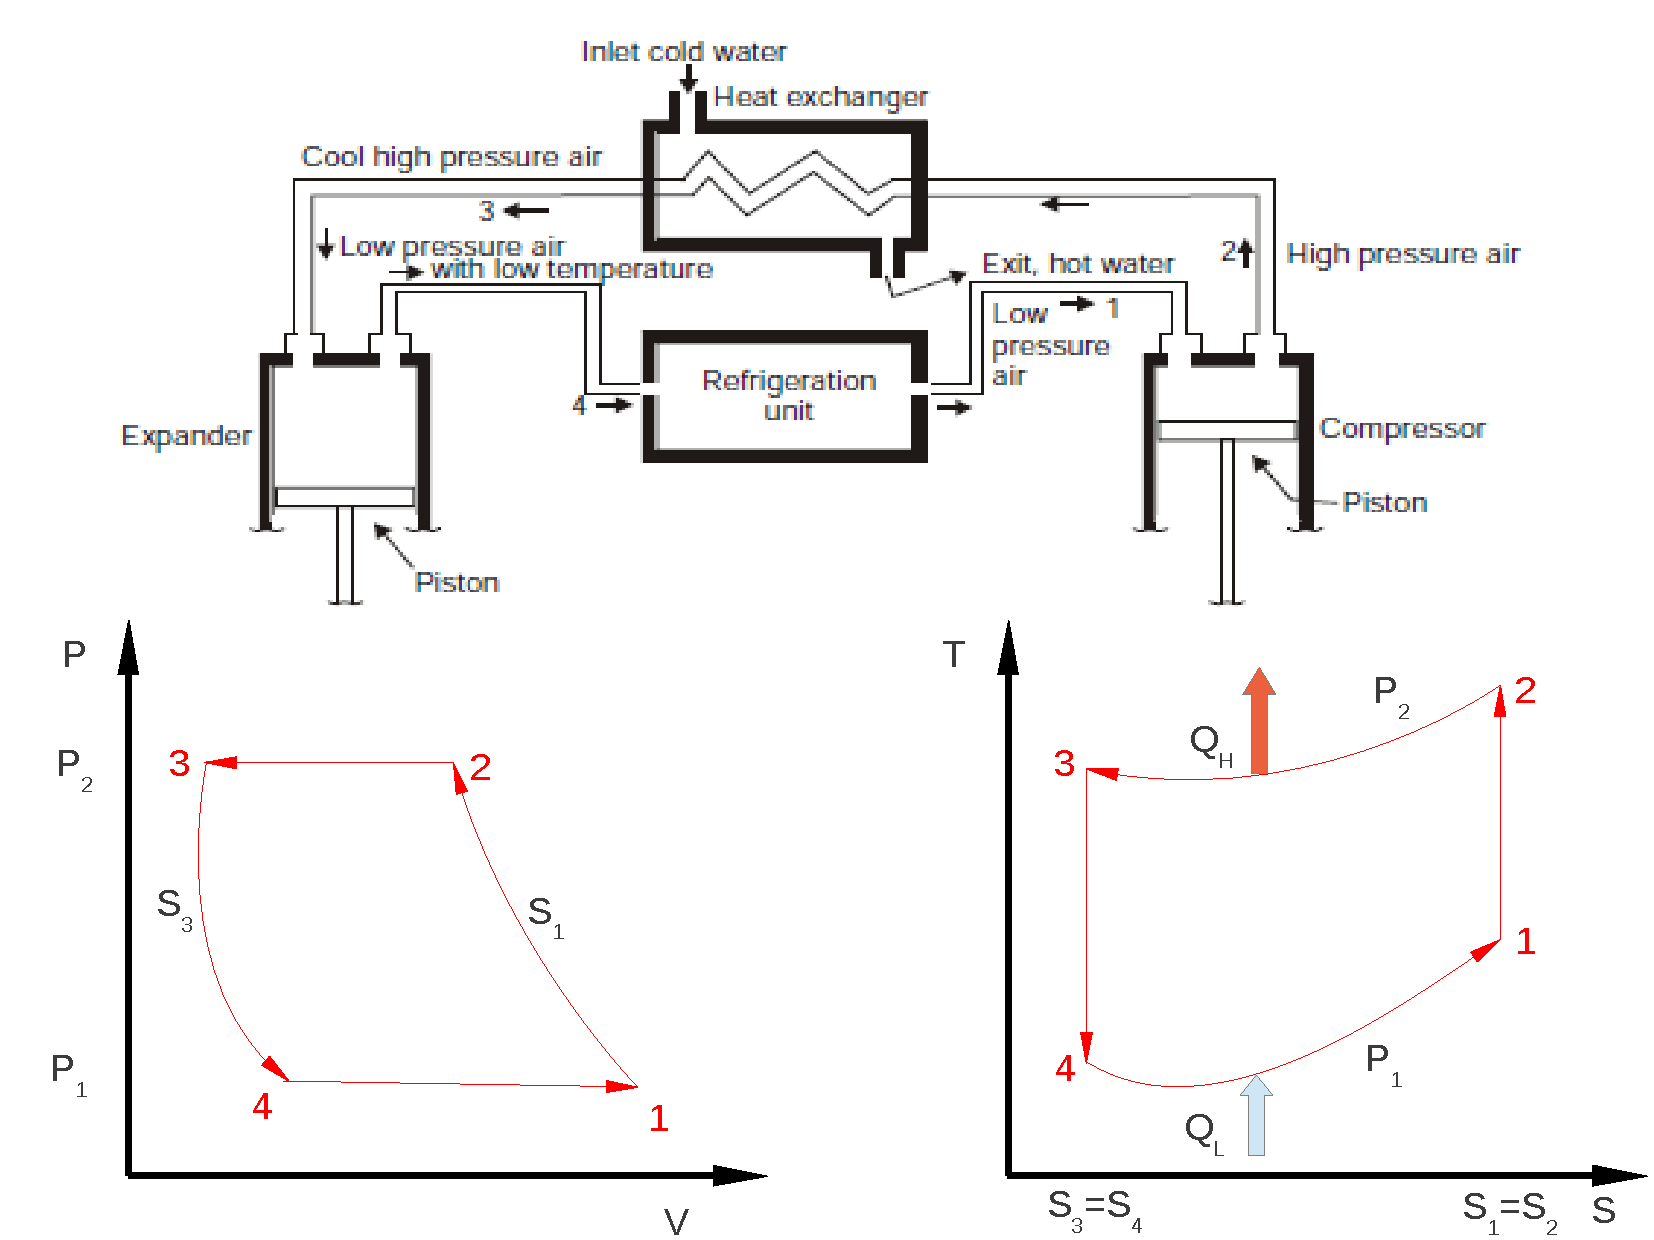
\includegraphics[width=8.3cm,height=7.6cm]{./Pics/Overview_Refrig6}
     \end{center}
    \end{figure}  
\end{frame}

%%%
%%% Slide
%%%
\begin{frame}
 \frametitle{Bell-Coleman Cycle (or Reversed Brayton Cycle)}
  \begin{columns}

   \begin{column}[c]{0.55\linewidth}
    \begin{figure}%
     \begin{center}
      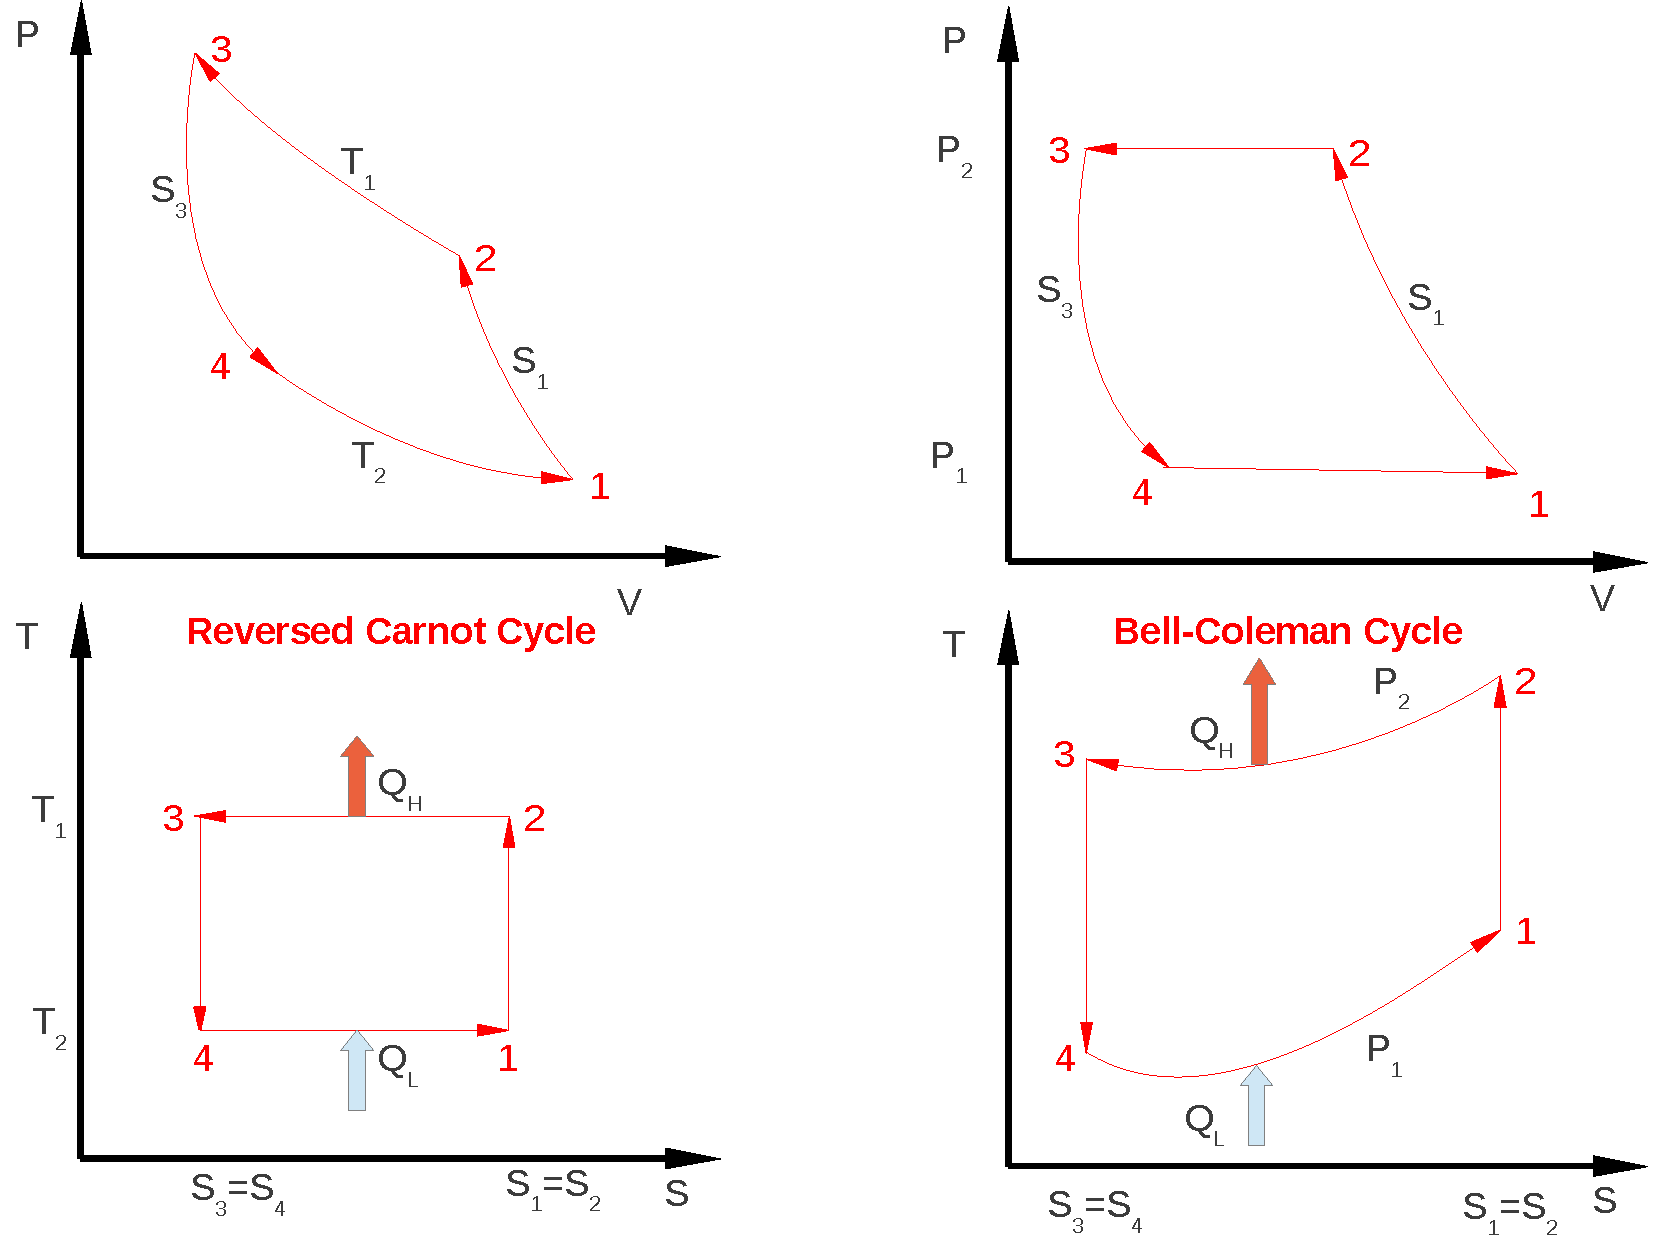
\includegraphics[width=6.8cm,height=6.cm]{./Pics/Overview_Refrig7}
     \end{center}
    \end{figure}  
   \end{column}  


   \begin{column}[c]{0.45\linewidth}
    \begin{enumerate}[(a)]
     \item <1-> Bell-Coleman Cycle uses air as a refrigerant and is a modified form of reversed Carnot cycle where;
     \item <2-> Isothermal heat addition and release are replaced by isobaric processes;
     \item <3-> Mostly used in cargo ships and aircraft refrigeration;
     \item <4-> The process involves compressor, heat exchanger, expander and refrigeration unit.
    \end{enumerate}
   \end{column}
  \end{columns}


\end{frame}



%%%
%%% Slide
%%%
\begin{frame}
 \frametitle{Bell-Coleman Cycle (or Reversed Brayton Cycle)}
  \begin{columns}

   \begin{column}[c]{0.55\linewidth}
    \begin{figure}%
     \begin{center}
      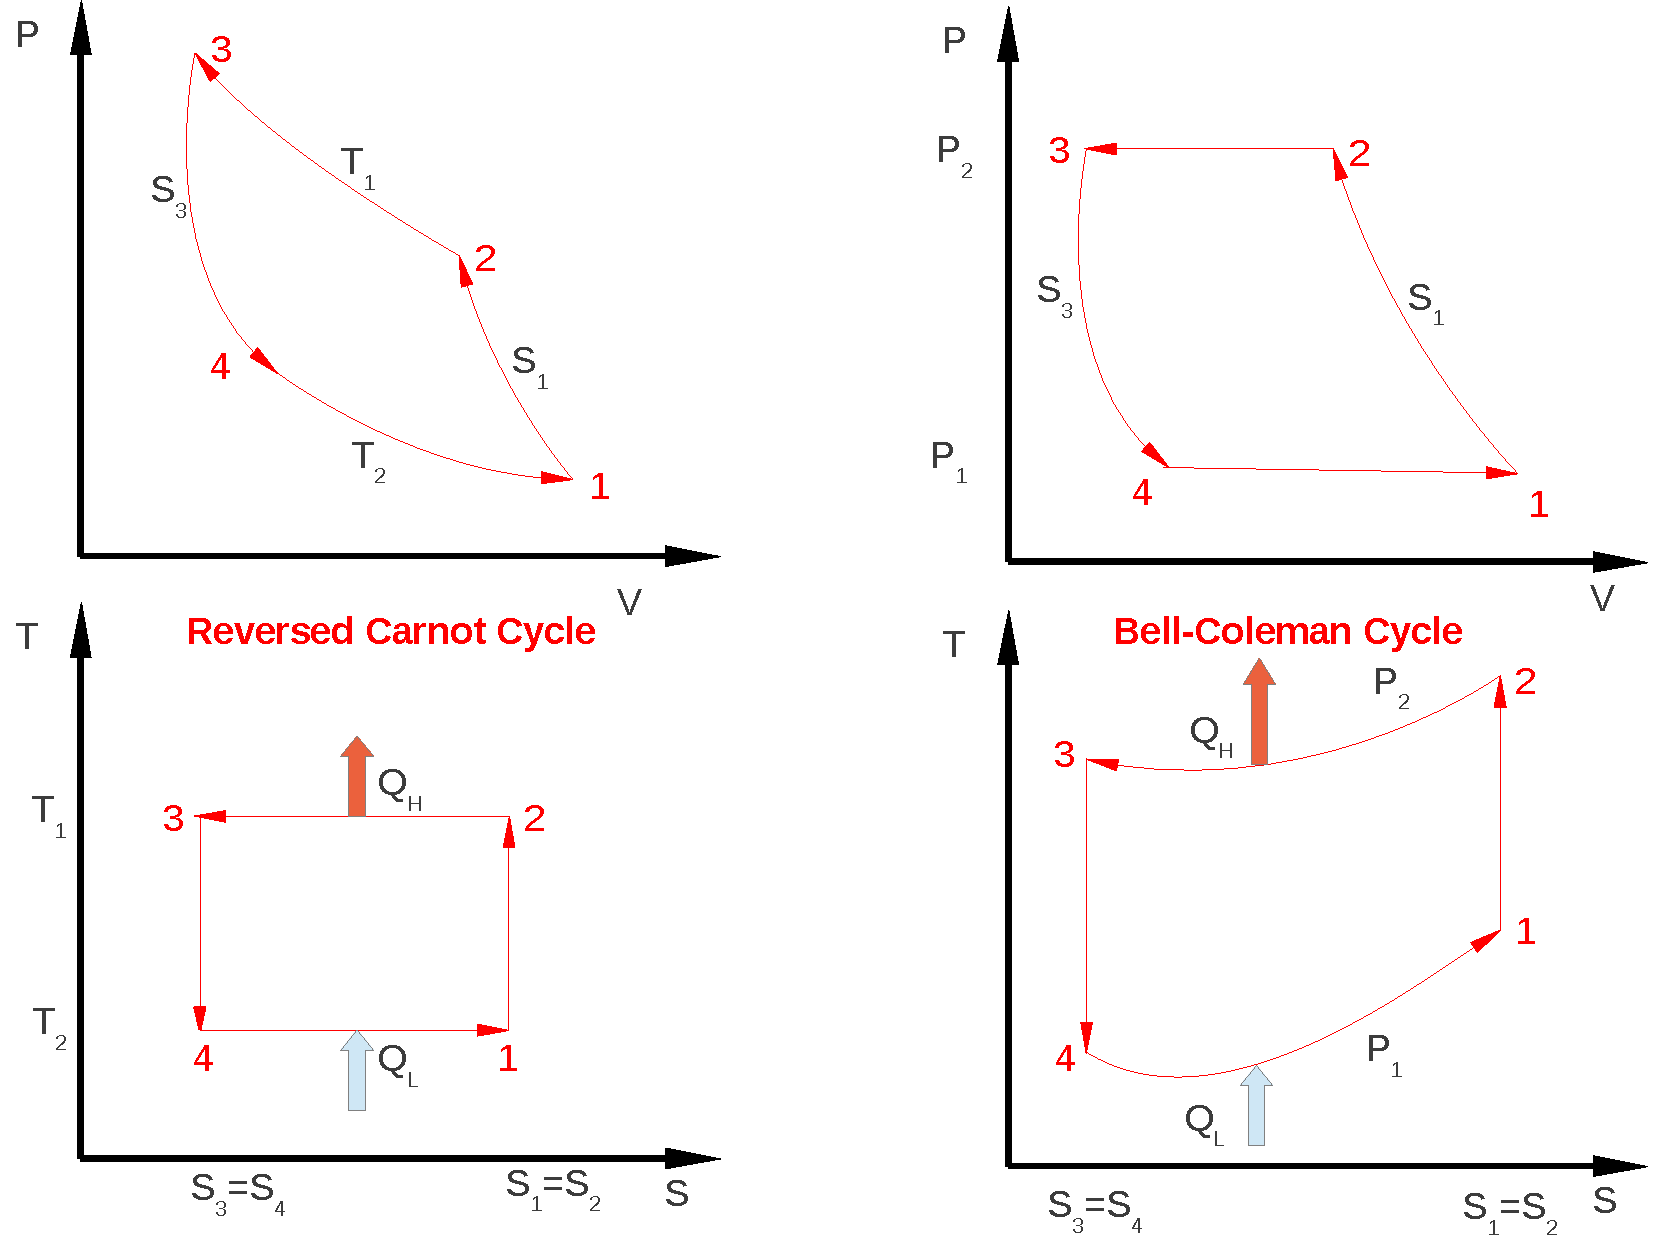
\includegraphics[width=6.8cm,height=6.cm]{./Pics/Overview_Refrig7}
     \end{center}
    \end{figure}  
   \end{column}  


   \begin{column}[c]{0.45\linewidth}
    \begin{itemize}
     \item <1-> \textcolor{blue}{1--2:} Adiabatic compression of air;
     \item <2-> \textcolor{blue}{2--3:} Isobaric heat rejection:
      \begin{displaymath}
       Q_{\text{rejected}}=mC_{p}\left(T_{2}-T_{3}\right)
      \end{displaymath}
     \item <3-> \textcolor{blue}{3--4:} Adiabatic expansion;
     \item <4-> \textcolor{blue}{4--1:} Isobaric heat absorption:
      \begin{displaymath}
       Q_{\text{absorbed}}=mC_{p}\left(T_{1}-T_{4}\right)
      \end{displaymath}
    \end{itemize}
   \end{column}
  \end{columns}


\end{frame}


%%%
%%% Slide
%%%
\begin{frame}
 \frametitle{Thermodynamic Analysis}
    \begin{itemize}
     \item <1-> The net work done upon system,
      \begin{eqnarray}
       W &=& \left(\text{Heat Rejected - Heat Absorbed}\right) \nonumber \\
         &=& mC_{p}\left(T_{2}-T_{3}\right) - mC_{p}\left(T_{1}-T_{4}\right)
      \end{eqnarray}
     \item <2-> Last lecture we defined the Coefficient of Performance as,
      \begin{eqnarray}
       \textcolor{blue}{\text{COP}} &=& \frc{\text{Desired Effect}}{\text{Net Work}} = \frc{mC_{p}\left(T_{1}-T_{4}\right)}{mC_{p}\left(T_{2}-T_{3}\right) - mC_{p}\left(T_{1}-T_{4}\right)} \nonumber \\
                  &=& \textcolor{blue}{\frc{1}{\left(\frc{T_{2}}{T_{1}}-\frc{T_{3}}{T_{4}}\right)-1} = \text{COP}_{\text{ideal}}}\label{refrig_CopIdeal}
      \end{eqnarray}
     \item <3-> Equation \ref{refrig_CopIdeal} describes the COP for \textcolor{blue}{ideal processes}. 
     \item <4-> In practice, the expansion and compression stages are described as \textcolor{blue}{polytropic: $PV^{n}$ = constant}, in which \textcolor{blue}{$n$} is assumed constant for each stage.
    \end{itemize}


\end{frame}


%%%
%%% Slide
%%%
\begin{frame}
 \frametitle{Thermodynamic Analysis}
    \begin{itemize}
     \item <1-> In \textcolor{blue}{Actual cycles}, the heat absorption and rejection stages may occur with some \textcolor{blue}{pressure loss} leading to a deviation of the isobaric process.
     \item <2-> The work required by compressor:
      \begin{displaymath}
       W_{\text{comp}} = \left[\frc{n}{n-1}\right] \left(P_{2}V_{2}-P_{1}V_{1}\right) = \left[\frc{n}{n-1}\right] R \left(T_{2}-T_{1}\right) \times m
      \end{displaymath}
     \item <3-> The work available from the expander:
      \begin{displaymath}
       W_{\text{exp}} = \left[\frc{n}{n-1}\right] \left(P_{2}V_{3}-P_{1}V_{4}\right) = \left[\frc{n}{n-1}\right] R \left(T_{3}-T_{4}\right) \times m
      \end{displaymath}
     \item <4-> And the actual net work, $W_\text{actual} = W_{\text{comp}} - W_{\text{exp}}$,
      \begin{displaymath}
       W_{\text{actual}} = m\left[\frc{n}{n-1}\right]R\left[\left(T_{2}-T_{1}\right)-\left(T_{3}-T_{4}\right)\right]
      \end{displaymath}
     \item <5-> Assuming $C_{p} = \frc{\gamma R}{\gamma - 1}$,
      \begin{equation}
       W_{\text{actual}} = m \left[\frc{n}{n-1}\right] C_{p} \left(\frc{\gamma - 1}{\gamma}\right) \left[\left(T_{2}-T_{1}\right)-\left(T_{3}-T_{4}\right)\right]
      \end{equation}
    \end{itemize}

\end{frame}


%%%
%%% Slide
%%%
\begin{frame}
 \frametitle{Thermodynamic Analysis}
    \begin{itemize}
     \item <1-> And the COP$_{\text{actual}}$ is calculated from,
      \begin{eqnarray}
       \textcolor{blue}{\text{COP}_{\text{actual}}} &=& \frc{ m C_{p}\left(T_{1}-T_{4}\right)} {m \left[\frc{n}{n-1}\right] C_{p} \left(\frc{\gamma - 1}{\gamma}\right) \left[\left(T_{2}-T_{1}\right)-\left(T_{3}-T_{4}\right)\right]} \nonumber \\
                               &=& \textcolor{blue}{\frc{1}{\left[\frc{n}{n-1}\right]\left[\frc{\gamma-1}{\gamma}\right]\left[\frc{T_{2}-T_{3}}{T_{1}-T_{4}}-1\right]}}
      \label{refrig_CopActual}
      \end{eqnarray}
     \item <2-> \textcolor{blue}{For isentropic processes, $\gamma=n$ and COP$_{\text{actual}}$=COP$_{\text{ideal}}$.}
     \item <3-> Assuming isentropic processes -- \textcolor{blue}{1--2} and \textcolor{blue}{3--4}: $\left[\frc{P_{2}}{P_{1}}\right]^{\frc{\gamma-1}{\gamma}}=\frc{T_{2}}{T_{1}}$ and $\left[\frc{P_{2}}{P_{1}}\right]^{\frc{\gamma-1}{\gamma}}=\frc{T_{3}}{T_{4}}$;
     \item <4-> The relationship above leads to: $\frc{T_{2}}{T_{1}}=\frc{T_{3}}{T_{4}}$, $\frc{T_{4}}{T_{1}}=\frc{T_{3}}{T_{2}}$ and $\frc{T_{1}-T_{4}}{T_{2}-T_{3}}=\frc{T_{1}}{T_{2}}$
    \end{itemize}

\end{frame}

%%%
%%% Slide
%%%
\begin{frame}
 \frametitle{Thermodynamic Analysis}
    \begin{itemize}
     \item <1-> Now replacing the previous relations into
     \item <2-> COP$_{\text{ideal}}$ (Eqn. \ref{refrig_CopIdeal}) and
      \begin{equation}
         \textcolor{blue}{\text{COP}_{\text{ideal}}} = \frc{1}{\left(\frc{T_{2}}{T_{1}}-\frc{T_{3}}{T_{4}}\right)-1} = \frc{1}{\frc{T_{2}}{T_{1}}-1} = \textcolor{blue}{\frc{T_{1}}{T_{2}-T_{1}}} 
      \end{equation}
     \item <3-> COP$_{\text{actual}}$ (Eqn. \ref{refrig_CopActual})
      \begin{eqnarray}
        \textcolor{blue}{\text{COP}_{\text{actual}}} &=& \frc{1}{\left[\frc{n}{n-1}\right]\left[\frc{\gamma-1}{\gamma}\right]\left[\frc{T_{2}-T_{3}}{T_{1}-T_{4}}-1\right]} \nonumber \\
         &=& \textcolor{blue}{\frc{T_{1}}{\left[\frc{n}{n-1}\right]\left[\frc{\gamma-1}{\gamma}\right]\left(T_{2}-T_{1}\right)}}
      \end{eqnarray}
    \end{itemize}

\end{frame}


%%%
%%% Slide
%%%
\begin{frame}
 \frametitle{Thermodynamic Analysis}
  \begin{columns}

   \begin{column}[c]{0.55\linewidth}
    \begin{figure}%
     \begin{center}
      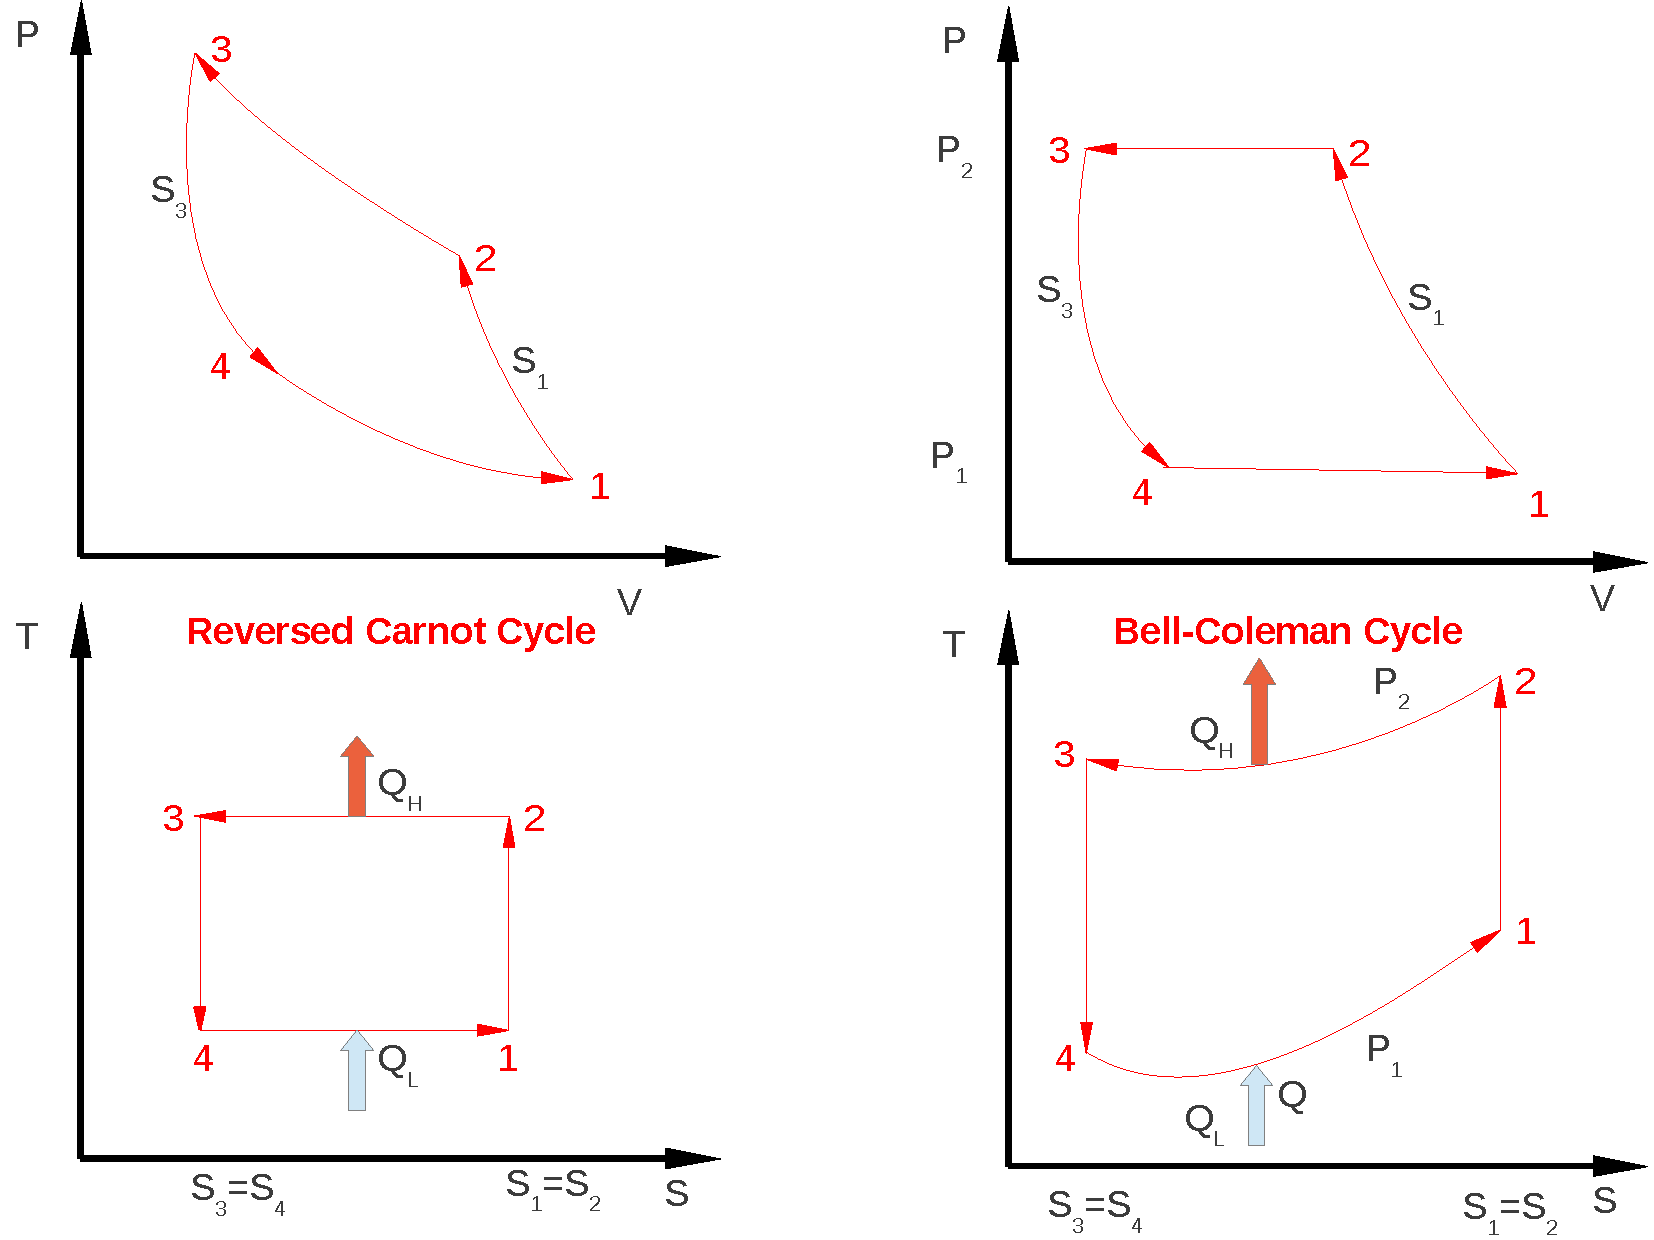
\includegraphics[width=6.8cm,height=6.cm]{./Pics/Overview_Refrig8}
     \end{center}
    \end{figure}  
   \end{column}  


   \begin{column}[c]{0.45\linewidth}
    \begin{itemize}
     \item <1-> From $PV$ and $TS$ diagrams, the $\text{COP}_{\text{Carnot}}=\frc{T_{1}}{T_{3}-T_{1}}$;
     \item <2-> As $T_{2}>T_{3}$, comparing the ideal Bell-Coleman cycle and the reversed Carnot cycle, $\Longrightarrow$ \textcolor{blue}{COP$_{\text{BC}}$ $<$ COP$_{\text{Carnot}}$};
     %\item <3-> 
    \end{itemize}
   \end{column}
  \end{columns}

\end{frame}


%%%
%%% Slide
%%%
\begin{frame}
 \frametitle{Example 1: Bell-Coleman Cycle (Reversed Brayton Cycle)}
\textcolor{blue}{{\it A refrigerating engine operates on the Bell-Coleman cycle with upper limiting pressure of 5.2 bar. Pressure and temperature at the beginning of the compression stage are 1.0 bar and 16$^{\text{o}}$C, respectively. The compressed air is cooled at constant pressure from a temperature of 41$^{\text{o}}$C  (flow entering the expansion cylinder). Assuming that both expansion and compression processes are adiabatic with $\gamma=1.4$ and the latent heat of fusion of water $\left(\text{L}_{\text{f}}\right)$ is 336 kJ/kg determine:}}

\begin{enumerate}[(a)]
\item \textcolor{blue}{{\it COP;}}
\item \textcolor{blue}{{\it Mass flow rate of air in circulation (kg/min);}}
\item \textcolor{blue}{{\it Piston displacement of compressor and expander;}}
\item \textcolor{blue}{{\it Bore of compressor and expansion cylinders. The unit runs at 240 rpm. Assume that the stroke length is 200 mm;}}
\item \textcolor{blue}{{\it Power required to drive the unit.}}
\end{enumerate}

\end{frame}


%%%
%%% Slide
%%%
\begin{frame}
 \frametitle{Example 1: Bell-Coleman Cycle (Reversed Brayton Cycle)}
  \begin{columns}

   \begin{column}[c]{0.53\linewidth}
    \begin{figure}%
     \begin{center}
      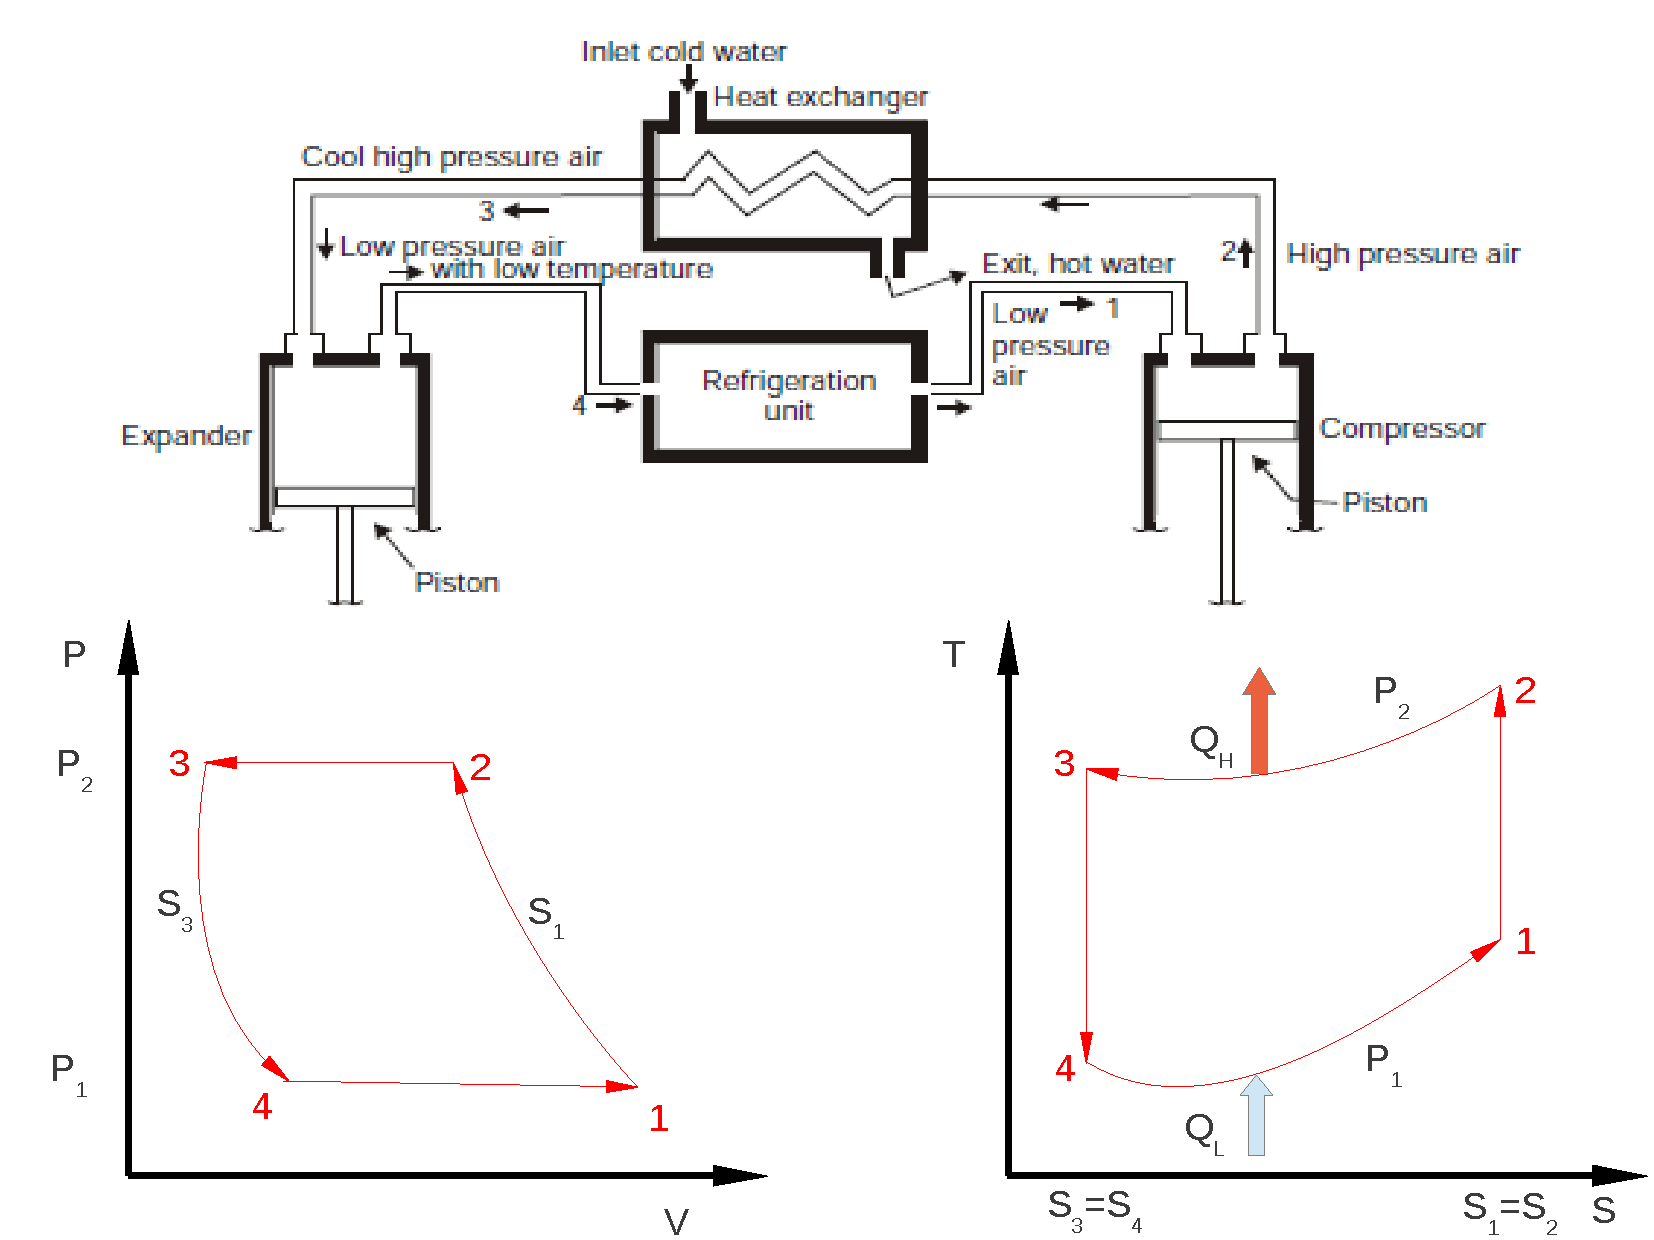
\includegraphics[width=6.8cm,height=6.cm]{./Pics/Overview_Refrig6}
     \end{center}
    \end{figure}  
   \end{column}  


   \begin{column}[c]{0.47\linewidth}
    Given: $T_{3}=314.15$ K, $T_{1}=289.15$ K, $P_{3}=P_{2}=5.2$ bar, $P_{4}=P_{1}=1.0$ bar, $\gamma=1.4$ and $C_{p}=1.003$ kJ/(kg.K).\\

    Assuming adiabatic compression $1-2$:
    \begin{eqnarray}
     \frc{T_{2}}{T_{1}}&=&\left(\frc{P_{3}}{P_{4}}\right)^{\frc{\gamma-1}{\gamma}} \nonumber \\
                      & =& \left(\frc{5.2}{1.0}\right)^{\frc{1.4-1}{1.4}} =1.60 \nonumber \\
                      &\Rightarrow& T_{2}= 463.12 \text{ K} = 189.97^{\text{o}}\text{C} \nonumber
    \end{eqnarray}

   Similarly the adiabatic expansion process $3-4$, $\frc{T_{3}}{T_{4}}=\left(\frc{P_{3}}{P_{4}}\right)^{\frc{\gamma-1}{\gamma}}$
   \end{column}
  \end{columns}

\end{frame}


%%%
%%% Slide
%%%
\begin{frame}
 \frametitle{Example 1: Bell-Coleman Cycle (Reversed Brayton Cycle)}
  \begin{itemize}
   \item <1-> Similarly for the adiabatic expansion process $3-4$, 
    \begin{displaymath}
     \frc{T_{3}}{T_{4}}=\left(\frc{P_{3}}{P_{4}}\right)^{\frc{\gamma-1}{\gamma}} \Rightarrow T_{4}=196.34\text{ K} = -76.81^{\text{o}}\text{C}
    \end{displaymath}

   \item <2-> In order to calculate the COP, 
    \begin{displaymath}
     \textcolor{blue}{\text{COP}} = \frc{T_{4}}{T_{3}-T_{4}} = \frc{196.34}{314.15-196.34} = \textcolor{blue}{1.67}
    \end{displaymath}

   \item <3-> The mas flow rate of air in circulation:
    \begin{eqnarray}
     \text{Refrigerating Effect per kg of air} &=& C_{p}\left(T_{1}-T_{4}\right) = 1.003\left(289.15-196.34\right) \nonumber \\
                                       &=& 93.09\text{ kJ/kg} \nonumber  
    \end{eqnarray}

    \item <4-> Remember that \textcolor{red}{1 tonne of Refrigeration (TR)} = $\frc{L_{f} \times \text{ 1 ton}}{ 1 day }$ = 336$\left[\frc{\text{ kJ}}{\text{kg}}\right]$ $\times$ $1000$ kg $\frc{1}{24\text{ hours}}$ = 14000 kJ/h
  \end{itemize}

\end{frame}




%%%
%%% Slide
%%%
\begin{frame}
 \frametitle{Example 1: Bell-Coleman Cycle (Reversed Brayton Cycle)}
  \begin{itemize}
   \item <1-> Thus, the Refrigerating Effect produced by the refrigerant engine (unit conversion): 6 \textcolor{blue}{TR} = 84000 kJ/h

%$6\left[\text{TR}\right] \times$ $\frc{14000 \text{kJ}}{\text{h}}$ $\frc{\text{kJ/h}}{\text{1 TR}}$ = $84000$ kJ/h

   \item <2-> Thus the \textcolor{blue}{mass flow rate of air in circulation}: $\frc{84000}{93.09\times 60}=$ \textcolor{blue}{$15.04$ kg/min}

   \item <3-> The piston displacement of the compressor is $V_{1}$ and defined as
     \begin{displaymath}
      \textcolor{blue}{V_{1}} =  \frc{m R T_{1}}{P_{4}} = \frc{15.04 \times 287 \times 289.15}{1.0\times 10^{5}} = \textcolor{blue}{12.48 \text{ m}^{3}/\text{kg}}
     \end{displaymath}

   \item <4-> The swept volume per stroke: $\frc{12.48}{240}=0.052$ m$^{3}$.

   \item <5-> We studied in Module 1 that the swept volume per stroke is defined as,
     \begin{displaymath}
      V_{s}^{\text{comp}}= \frc{\pi d_{c}^{2}}{4}\times l_{s} = \frc{\pi d_{c}^{2}}{4}\left(0.2\right) = 0.052 \Rightarrow \textcolor{blue}{d_{c} = 0.575\text{ m}}
     \end{displaymath}
    where $d_{c}$ is the diameter or bore of the compressing cylinder and $l_{s}$ is the length of the stroke

  \end{itemize}

\end{frame}




%%%
%%% Slide
%%%
\begin{frame}
 \frametitle{Example 1: Bell-Coleman Cycle (Reversed Brayton Cycle)}
  \begin{itemize}
   \item <1-> The piston displacement of the expander is $\textcolor{blue}{V_{4}}=\frc{m R T_{4}}{P_{4}} =$ \textcolor{blue}{8.476 m$^{3}$/min}
   \item <2-> And similarly for the  calculation of the swept volume per stroke in the compressor cylinder, for the expander: $\frc{8.476}{240}=0.035$ m$^{3}$.
     \begin{displaymath}
      V_{s}^{\text{exp}}= \frc{\pi d_{e}^{2}}{4}\times l_{s} = \frc{\pi d_{e}^{2}}{4}\left(0.2\right) = 0.035 \Rightarrow \textcolor{blue}{d_{e} = 0.474\text{ m}}
     \end{displaymath}
   \item <3-> Finally the power to drive the unit is
     \begin{eqnarray}
      && \text{COP}=\frc{\text{Refrigerant Effect}}{\text{Work done}} = 1.67 = \frc{ 6 \times 14000}{W} \nonumber \\
      &&\textcolor{blue}{W} = 50299.4 \text{ kJ/h} = 13.97 kJ/s = \textcolor{blue}{13.97 \text{kW}} \nonumber 
     \end{eqnarray}

  \end{itemize}

\end{frame}



\subsection{Reversed Stirling Cycle Refrigeration}
%%%
%%% Slide
%%%
\begin{frame}
 \frametitle{Reversed Stirling Refrigeration}
  \begin{itemize}
   \item <1-> In Module 01 we studied the Stirling thermal engine cycle that comprises two constant temperature processes and two constant volume processes;
   \item <2-> The reversed Stirling cycle operates with the same set of stages;
   %\item 
  \end{itemize}

    \begin{figure}%
     \begin{center}
      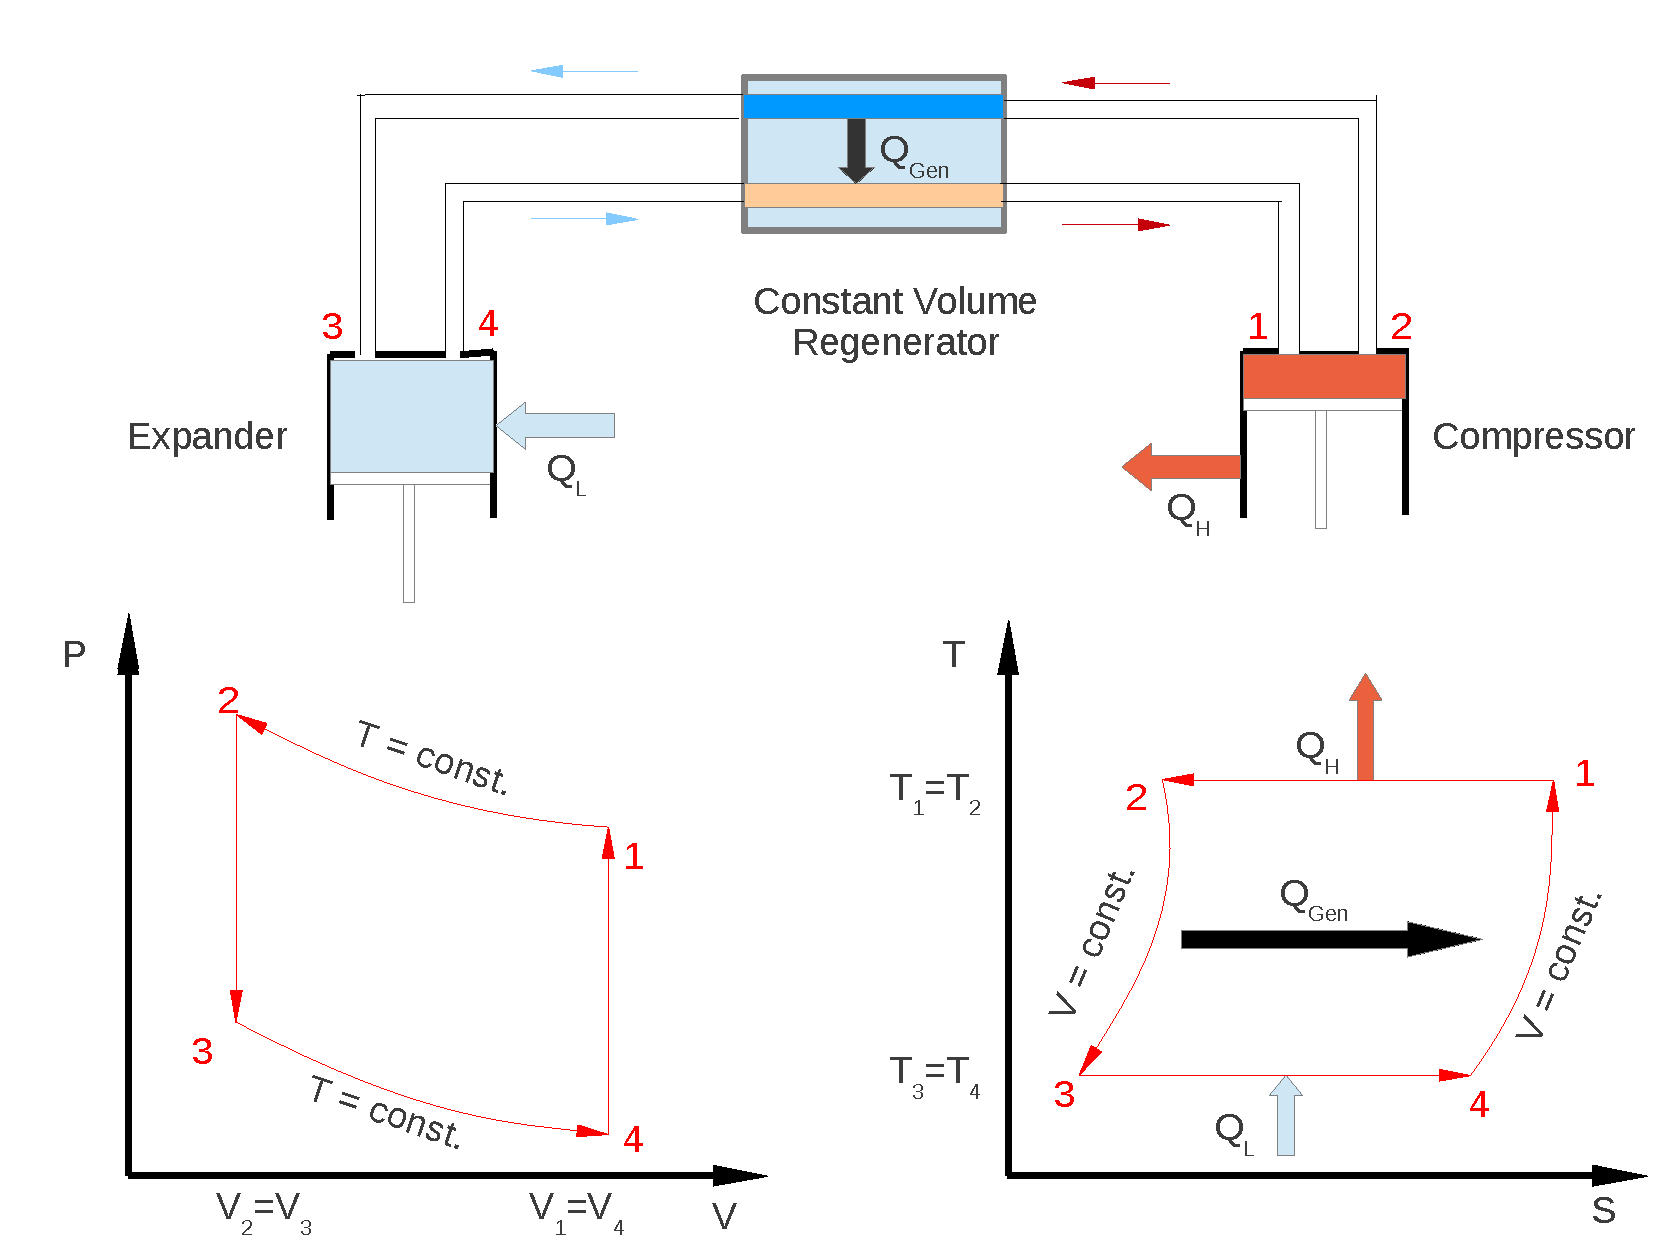
\includegraphics[width=8.3cm,height=6.0cm]{./Pics/Overview_Refrig9}
     \end{center}
    \end{figure}  

   %\item <4-> 
   %\item <5-> 
   %\item <6-> 
\end{frame}


%%%
%%% Slide
%%%
\begin{frame}
 \frametitle{Reversed Stirling Refrigeration}
  \begin{columns}

   \begin{column}[c]{0.55\linewidth}
    \begin{figure}%
     \begin{center}
      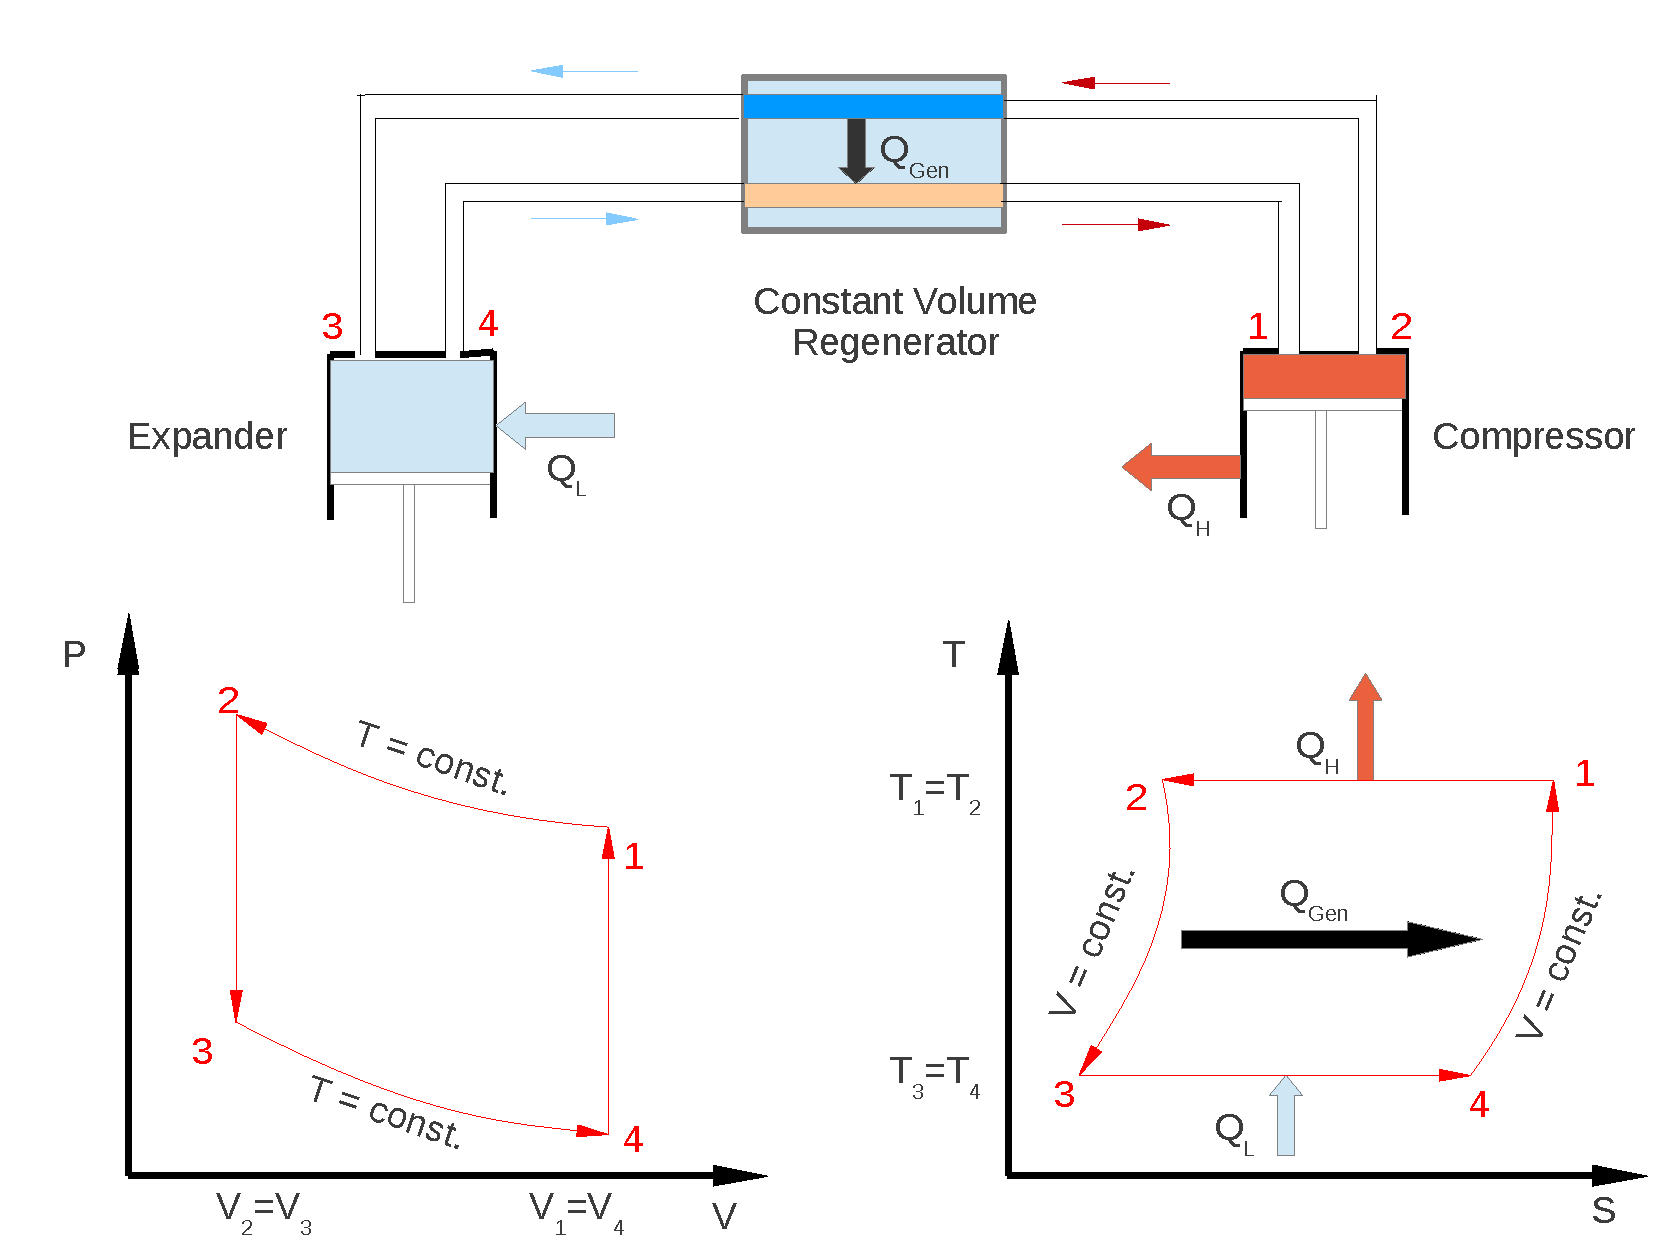
\includegraphics[width=6.8cm,height=6.cm]{./Pics/Overview_Refrig9}
     \end{center}
    \end{figure}  
   \end{column}  

   \begin{column}[c]{0.45\linewidth}
    \begin{enumerate}[(a)]
     \item <1-> In reversed Stirling Refrigeration cycles, reciprocating piston is the most effective mechanism used in which;
     \item <2-> Constant volume processes are approximated by the relatively small piston motion near the TDC and BDC crankshaft positions;
     \item <3-> As \textcolor{blue}{Stirling and Carnot cycles have the same thermal efficiency}, the \textcolor{red}{reversed Stirling and reversed Carnot cycles have the same coefficient of performance}.
    \end{enumerate}
   \end{column}

  \end{columns}
\end{frame}


%%%
%%% Slide
%%%
\begin{frame}
 \frametitle{Reversed Stirling Refrigeration}
  \begin{columns}

   \begin{column}[c]{0.55\linewidth}
    \begin{figure}%
     \begin{center}
      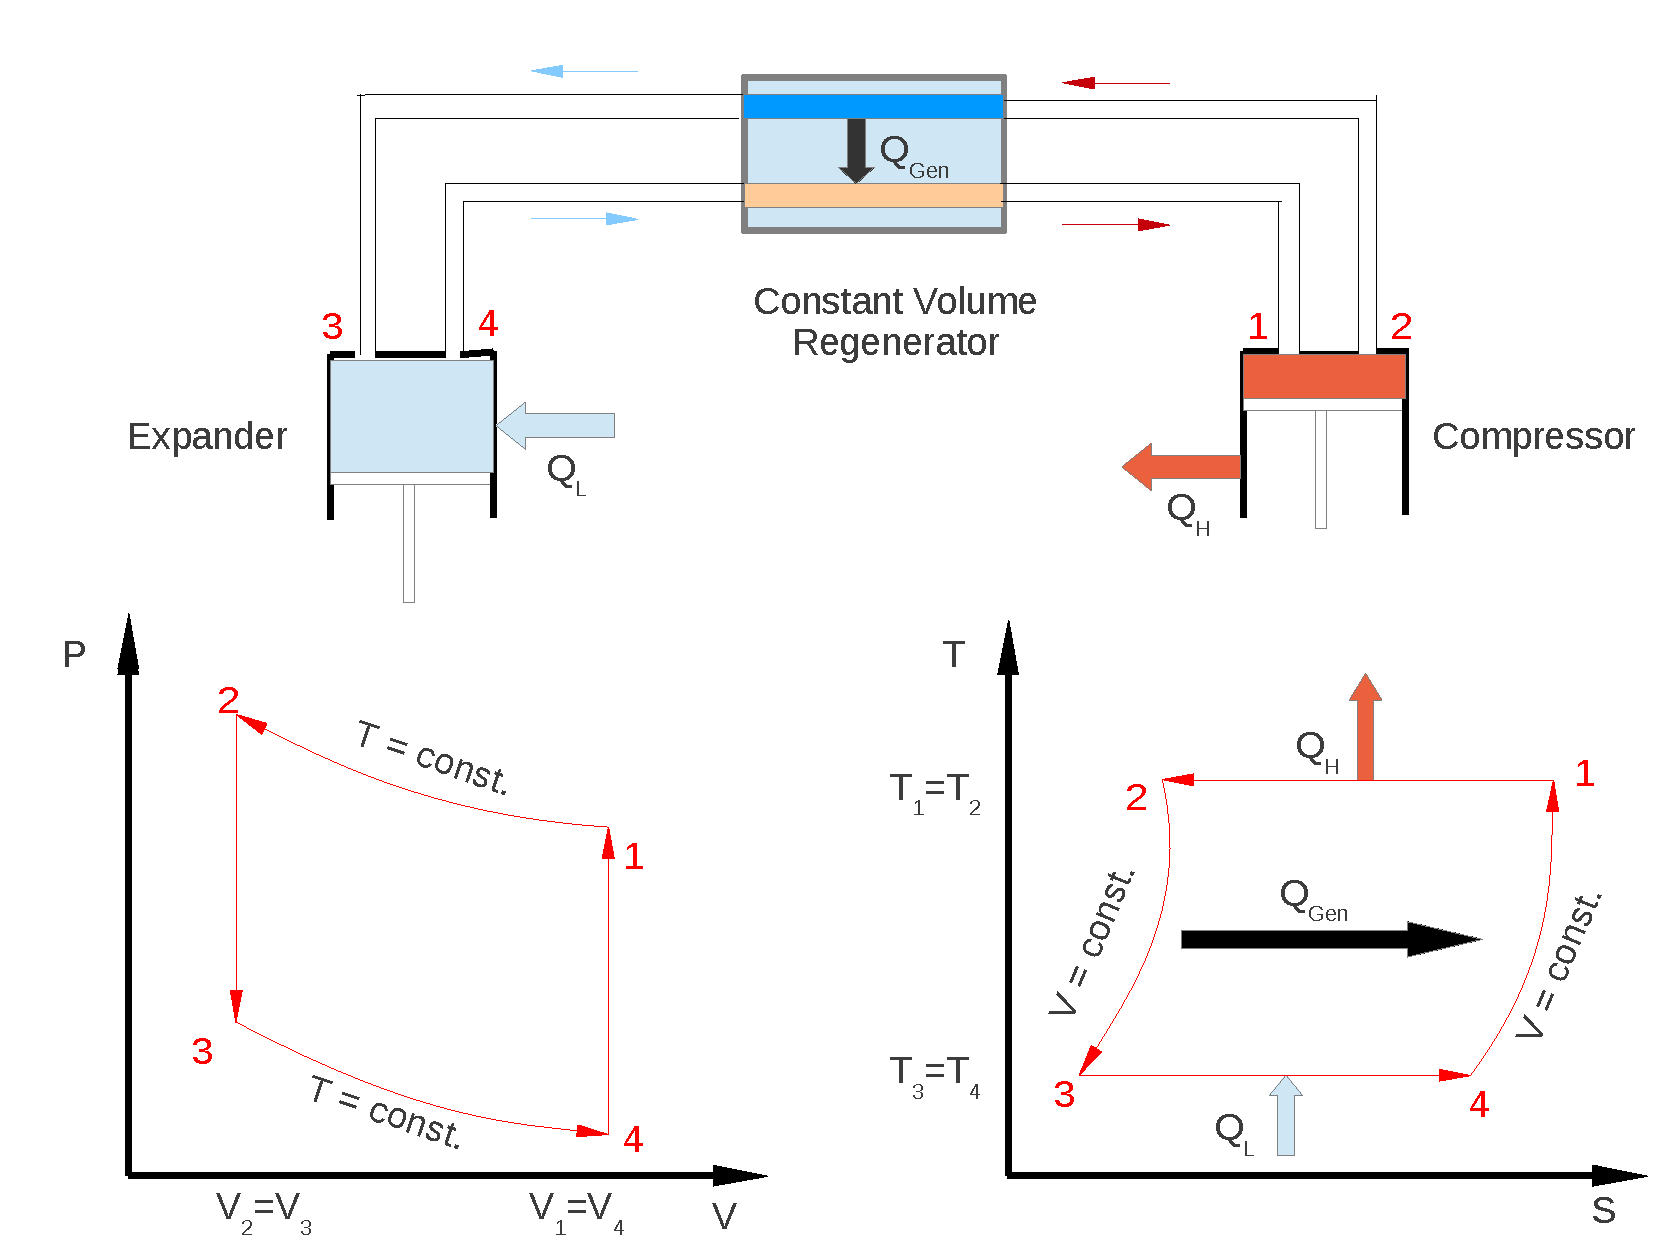
\includegraphics[width=6.8cm,height=6.cm]{./Pics/Overview_Refrig9}
     \end{center}
    \end{figure}  
   \end{column}  

   \begin{column}[c]{0.45\linewidth}
    \begin{enumerate}[(a)]
     \item <1-> \textcolor{blue}{1-2} is the isothermal compression with heat rejection Q$_{H}$ to the surroundings at temperature T$_{1}$=T$_{2}$;
     \item <2-> \textcolor{blue}{3-4} is the isothermal expansion with absorption Q$_{L}$ from the cold body at temperature T$_{3}$=T$_{4}$;
     \item <3-> \textcolor{blue}{2-3} and \textcolor{blue}{4-1} are constant volume heat transfer processes -- Q$_{2}^{3}$=Q$_{4}^{1}$;
     %\item <4-> If a perfect regenerator is employed between the cooling \textcolor{blue}{2-3} and heating \textcolor{blue}{4-1} processes, then  
    \end{enumerate}
   \end{column}

  \end{columns}
\end{frame}


%%%
%%% Slide
%%%
\begin{frame}
 \frametitle{Reversed Stirling Refrigeration}
  \begin{columns}

   \begin{column}[c]{0.55\linewidth}
    \begin{figure}%
     \begin{center}
      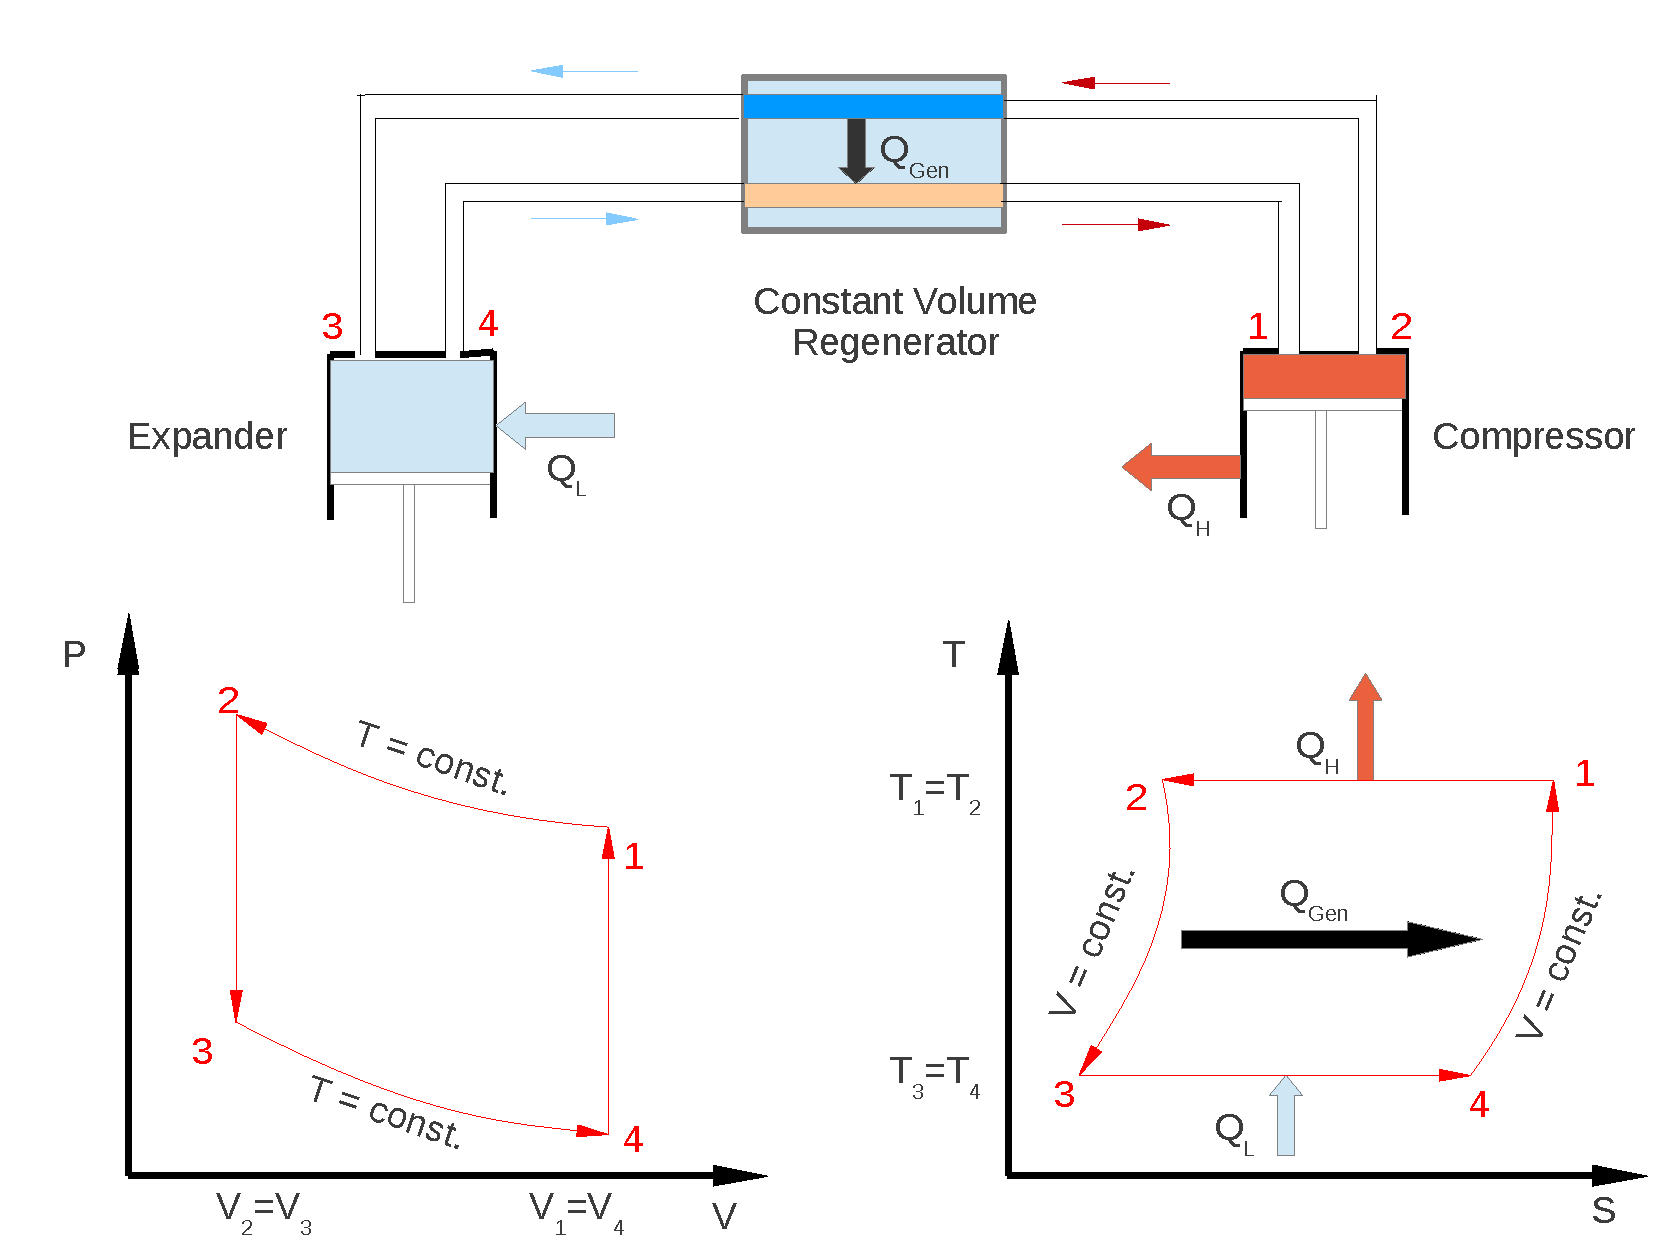
\includegraphics[width=6.8cm,height=6.cm]{./Pics/Overview_Refrig9}
     \end{center}
    \end{figure}  
   \end{column}  

   \begin{column}[c]{0.45\linewidth}
    \begin{enumerate}[(a)]
     \item <1-> Coefficient of Performance for refrigeration and heat pump:
      \begin{eqnarray}
       && COP_{R} = \frc{T_{L}}{T_{H}-T_{L}} \nonumber \\
       && COP_{HP} = \frc{T_{H}}{T_{H}-T_{L}} \nonumber
      \end{eqnarray} 
     \item <2-> The reversed Stirling cycle (RSC) has the same limitations of the Carnot cycle as it is very difficult to achieve isothermal compression and expansion processes with a real gas;
     \item <3-> However, RSC is not very dependent on the internal efficiencies of the compressor and the expander. 
    \end{enumerate}
   \end{column}

  \end{columns}
\end{frame}



%%%
%%% Slide
%%%
\begin{frame}
 \frametitle{Reversed Stirling Refrigeration}
  \begin{columns}

   \begin{column}[c]{0.55\linewidth}
    \begin{figure}%
     \begin{center}
      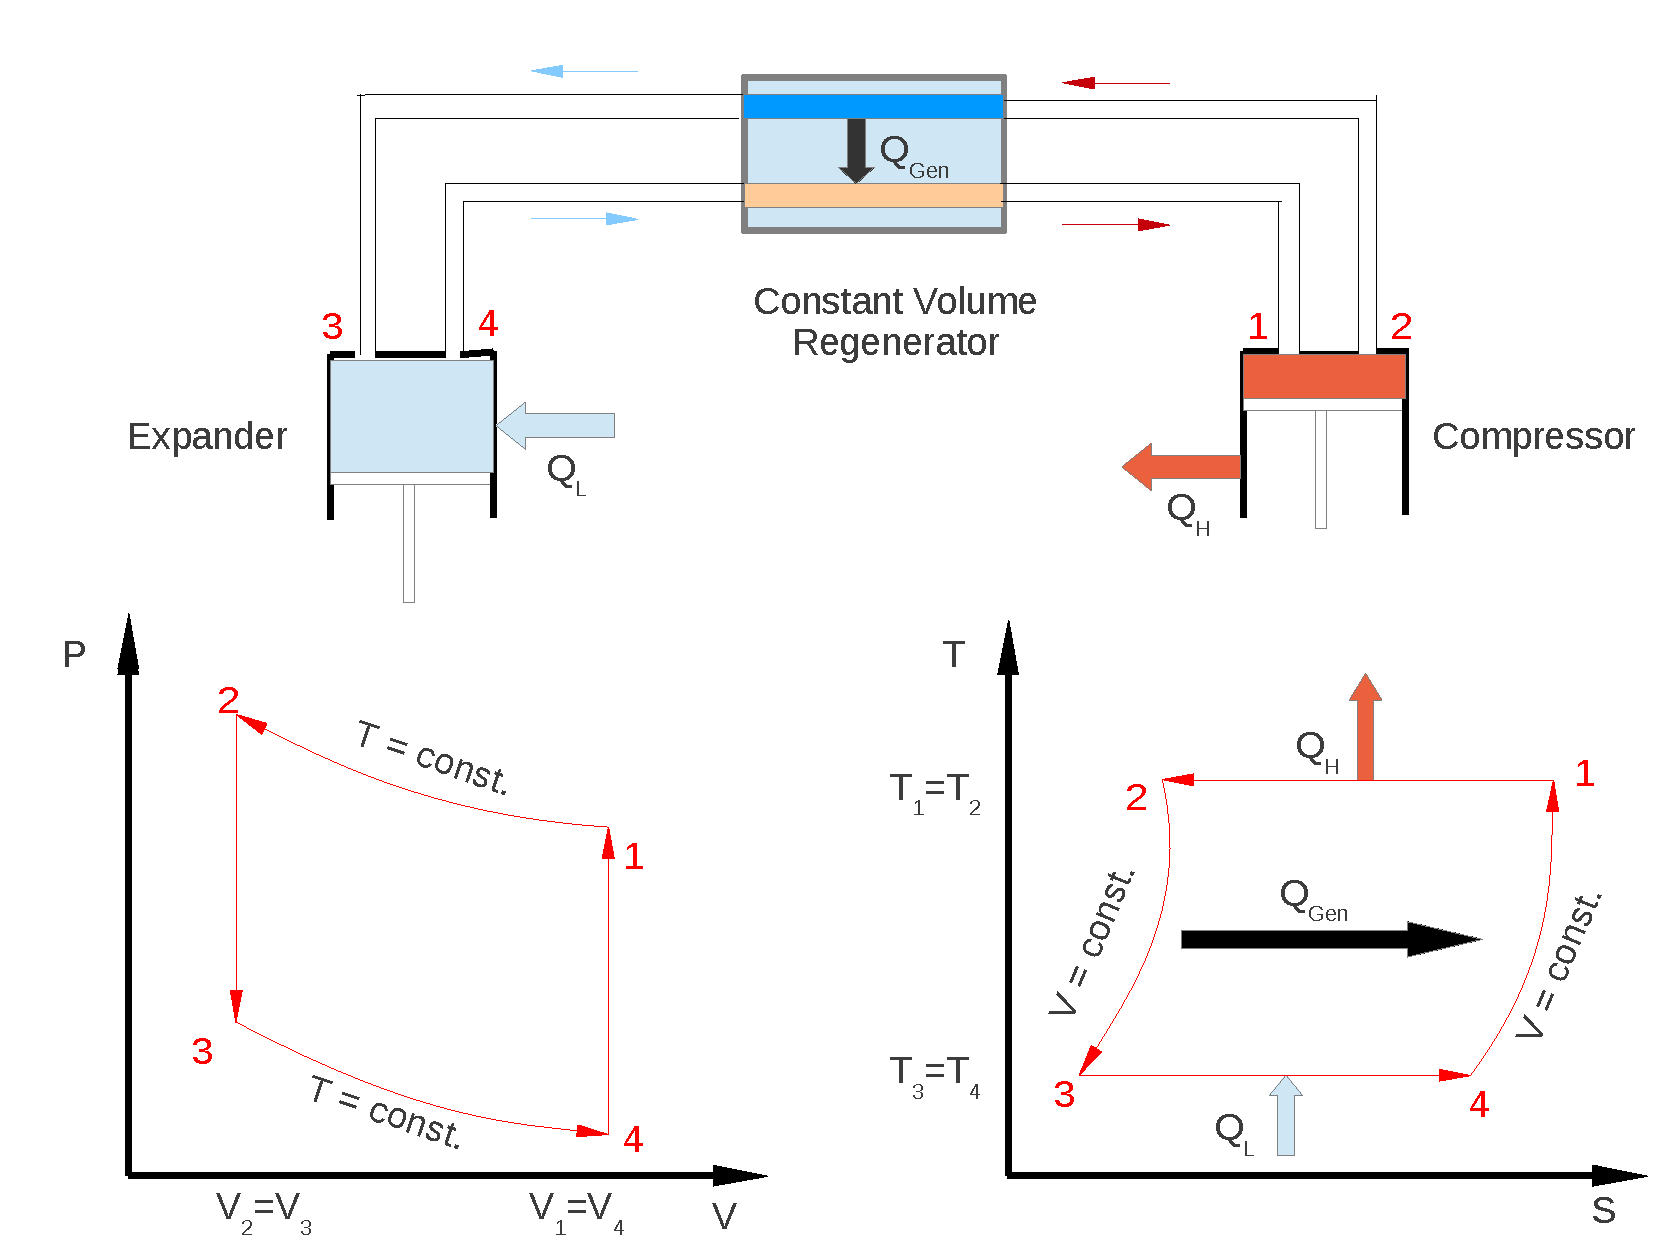
\includegraphics[width=6.8cm,height=6.cm]{./Pics/Overview_Refrig9}
     \end{center}
    \end{figure}  
   \end{column}  

   \begin{column}[c]{0.45\linewidth}
    \begin{enumerate}[(a)]
     \item <1-> In the \textcolor{blue}{Actual RSC}, the \textcolor{red}{regenerator} acts as perfect storage of heat and cold. 
     \item <2-> The major factors for COP in RSC are
       \begin{enumerate}[(i)]
        \item <3-> High regenerator efficiency;
        \item <4-> High heat transfer coefficients in compressor and expander spaces;
        \item <5-> Low pressure drop in system;
        \item <6-> Low work of compression.
       \end{enumerate}
     \item <7->This means that we need a fluid that has \textcolor{blue}{high thermal conductivity} and \textcolor{blue}{high thermal diffusivity}. Also, it would be desirable a low viscosity and low ratio of specific heats.
    \end{enumerate}
   \end{column}

  \end{columns}
\end{frame}


%$\left(\text{m}^{2}/\text{s}\right)$
%%%
%%% Slide
%%%
\begin{frame}
 \frametitle{Reversed Stirling Refrigeration}
  \begin{itemize}
   \item <2-> As it can be seen, \textcolor{blue}{H$_{2}$} has the largest $\kappa$, lowest $\mu$ and a reasonably large $\alpha$ and therefore is the preferred gas for use in RSC.
  \end{itemize}

 \begin{center}
 \begin{table}
  \begin{tabular}{c c c c c}
      \hline
                 &  $\kappa$   &  $\mu\times$ 10$^{-5}$ &  $\alpha \times$ 10$^{-4}$   & $\gamma$   \\
                 & (W/(m.K))   &  (kg/(m.s))           &  $\left(\text{m}^{2}/\text{s}\right)$ & \\
       \hline
       Air       & 0.02624     & 1.983                 & 0.2216        & 1.4 \\
      Hydrogen   &  0.182      & 0.8963                & 1.554         & 1.409  \\
     Helium      &  0.1491     & 2.012                 & 1.8           & 1.667 \\
   \hline            
  \end{tabular}
  \caption{$\kappa$: thermal conductivity, $\mu$: viscosity and $\alpha=\frc{\kappa}{\rho C_{p}}$: thermal diffusivity }
 \end{table}
\end{center}
\end{frame}



\section{Summary}

%%%
%%% Slides
%%%
\begin{frame}
 \frametitle{Summary -- Comparison between Gas-Refrigeration Cycles}

    \begin{figure}%
     \begin{center}
      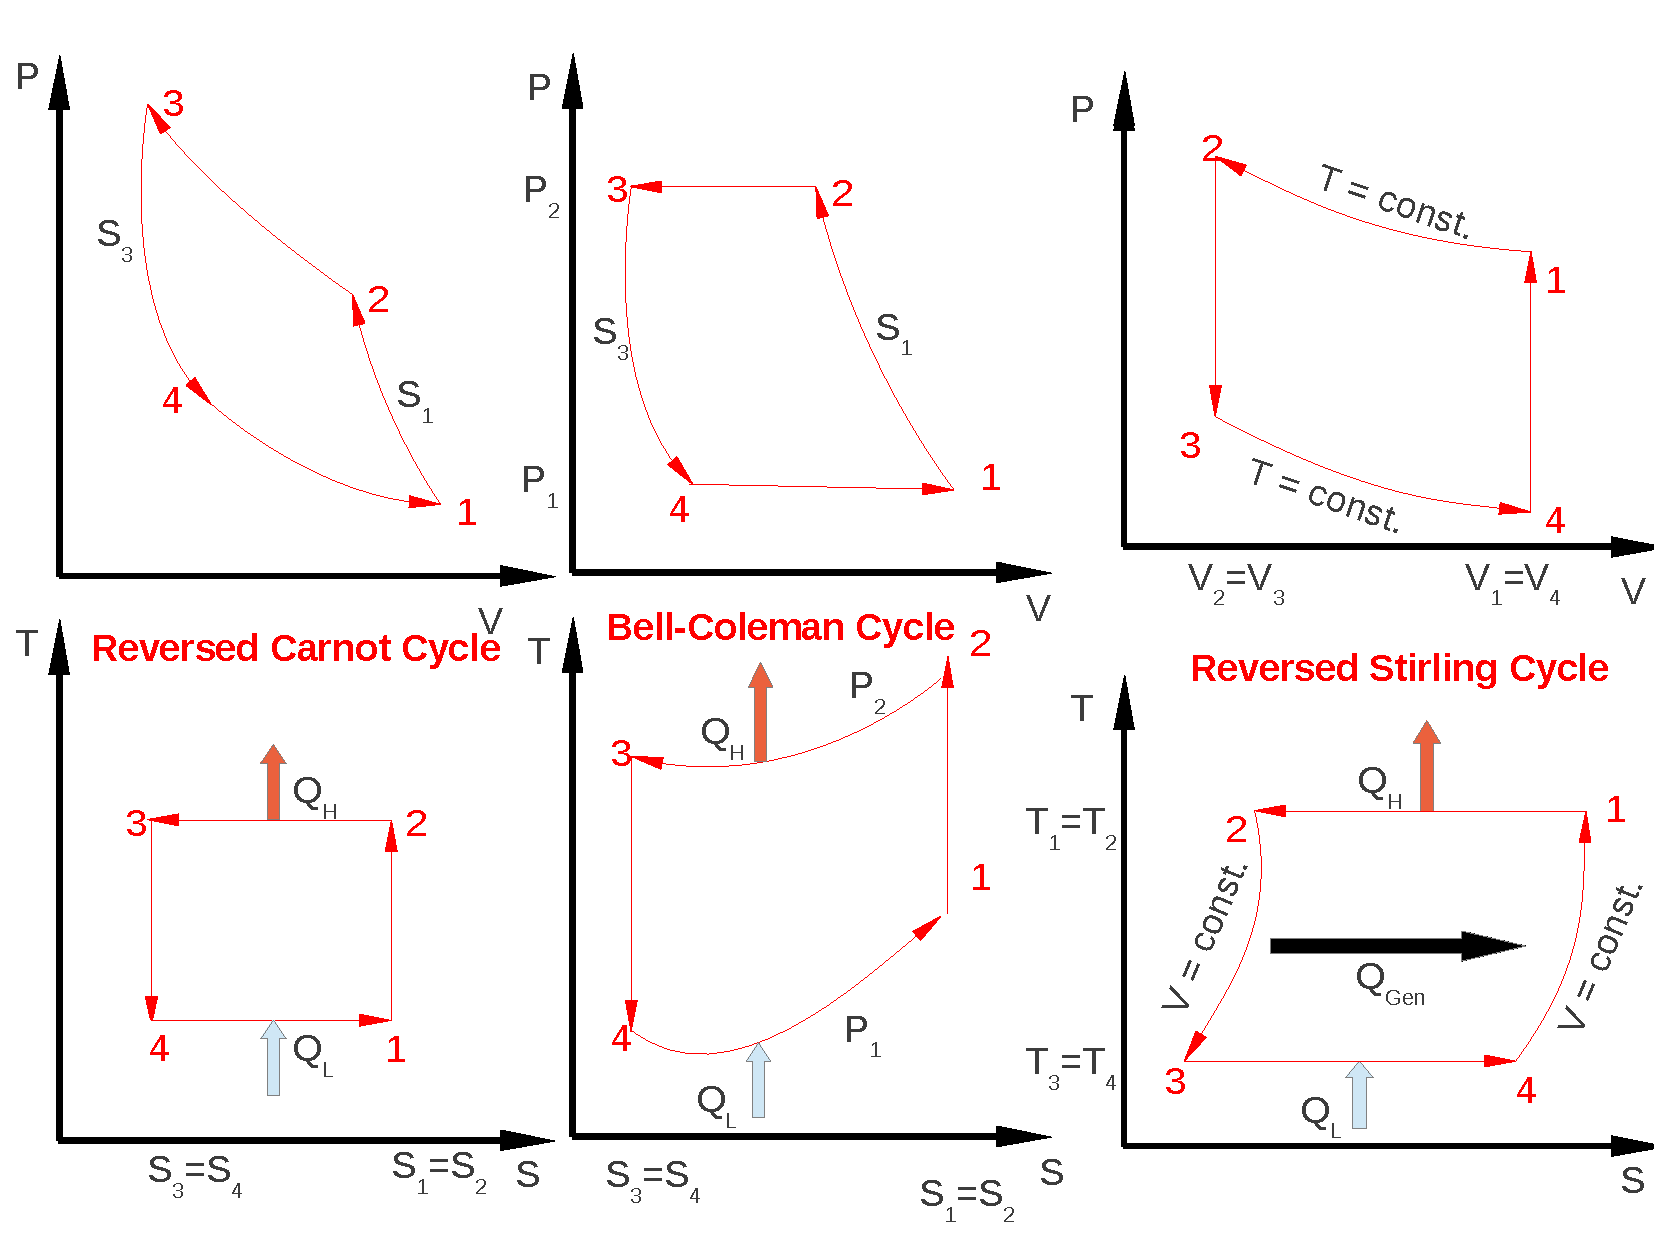
\includegraphics[width=11.5cm,height=7.8cm]{./Pics/Overview_Refrig10}
     \end{center}
    \end{figure}  

\end{frame}

%%%
%%% Slides
%%%
\begin{frame}
 \frametitle{Summary}
  After this lecture you should:
 \begin{enumerate}[(a)]
  \item <1-> Be able to draw the assumptions for the gas-refrigeration air-standard cycle;
  \item <2-> Understand the specific stages of the Reversed Brayton cycle (Bell-Coleman cycle) and the Reversed Stirling cycle and perform thermal analysis.
 \end{enumerate}
\end{frame}



\end{document}
